\section{Cryogenic \glsentryshort{sipm} Light Readout}
\label{sec:studies_viper-light-ro}

\glsreset{pmt}
\glsreset{sipm}

For the \AC{} detector concept, detailed in Section~\ref{sec:ac_argoncube}, a compact light readout is needed.
\glspl{pmt} are not suitable because they occupy a lot of space and thus would require mounting on top of a module, which in turn would reduce their efficiency.
That is why the photon detectors of choice for such a detector are \glspl{sipm}.

A novel light readout system based on \glspl{sipm} in \lar{} was implemented for the \AC{} pixel demonstrator described in Section~\ref{sec:ac_viper}.
Acrylic rings placed in between the aluminium field shaping rings of the \gls{tpc} provide the light collection; their inner surfaces are machine-polished and coated with the \gls{wls} \gls{tpb}. 
The coating method is based on~\cite{TPBcoating}.
\SI{0.5}{\gram} of \gls{tpb} and \SI{0.5}{\gram} of acrylic flakes were dissolved in \SI{50}{\milli\liter} of toluene and then mixed with \SI{12}{\milli\liter} of ethanol, which serves to increase the coating homogeneity. 
Three layers of the coating were applied by hand with a fine brush. 

\SI{1}{\milli\metre} diameter \gls{wls} fibres, \emph{Kuraray Y11(200)M}~\cite{kuraray}, couple the acrylic rings to four \emph{Hamamatsu S12825-050P} \glspl{sipm}~\cite{crt_sipm} mounted close to the anode (see Figure~\ref{fig:viper_v1per}). 
The \glspl{sipm} and their front-end electronics were adapted from those developed at \gls{help} for the \glspl{crt} used in \uboone{} and the \sbnd{}~\cite{crt, crt_feb}.
Residing on the cryostat top flange at room temperature, the \gls{feb} is connected to the \glspl{sipm} via Teflon insulated coaxial cables.
For operation in \lar{} the \gls{sipm} bias voltages has to be reduced from $\approx \SI{70}{\volt}$ to \SI{53}{\volt}, in order to compensate for change of breakdown voltage.

The peak of scintillation light emission in \lar{} lies at \SI{128}{\nano\metre} (see Table~\ref{tab:lartpc_larprop}) while the sensitivity wavelength peak of the \gls{sipm} is at \SI{450}{\nano\metre}.
Therefore, the scintillation light needs to be shifted before it can be detected by the \glspl{sipm}.
This happens in two stages.
For the first shift \gls{tpb} is applied to the inside of the acrylic rings.
Their outside is not coated to reduce the collected amount of scintillation light that originates outside the \gls{tpc} while their inside is machined to optimise light collection.
\gls{tpb} absorbs the \SI{128}{\nano\metre} scintillation light and re-emits it with a peak at \SI{440}{\nano\metre}~\cite{tpb}.
The light emitted by the \gls{tpb} is then propagated through the acrylic and coupled into the \gls{wls} fibre which has an absorption peak at \SI{430}{\nano\metre} and an emission peak at \SI{476}{\nano\metre}.

In the \gls{feb} two coincidences $\qty(\land)$ of two out of four \glspl{sipm} are formed and combined by means of a logic \emph{OR} $\qty(\lor)$ operation.
The trigger pattern is thus
\begin{IEEEeqnarray}{rCl}
	T & = & \qty(S_1 \land S_2) \lor \qty(S_3 \land S_4)
\end{IEEEeqnarray}
for \glspl{sipm} $S_1$ through $S_4$.
To improve trigger purity we tried to change the firmware to trigger on the coincidence of all four fibres in the \gls{tpc}.
Due to a firmware bug however this was not successful.

The light readout scheme described above was successfully used to trigger and record several thousand cosmic muon interactions with the \AC{} pixel demonstrator, as will be explained in Section~\ref{sec:ac_viper}.
However, when compared to a measurement triggered on the charge readout directly, it became apparent that the efficiency of this light readout was very poor.
No quantitative measurement of the trigger efficiency was performed due to limitations in the experimental setup.
Triggering on the charge readout was only possible using an oscilloscope because the used \gls{daq} system was not capable of self-triggering.
Therefore, the channel number was limited to four which would have enabled charge readout triggering only on a subset of the readout area.
An external reference trigger source, such as a muon telescope, was not available during the measurements.
After warming up the experiment, we discovered that all four fibres were damaged because the acrylic rings had fallen out of their mounting brackets and squeezed or even broken the fibres.

Another drawback of the design is the optical coupling between the acrylic rings and the \lar{}.
A lot of light escapes from the rings and is lost because the refractive indices are very close.
Many other low-volume light readout systems based on light guides have been developed for \lar{}~\cite{lar_lro1, lar_lro2, lar_lro3, lar_lro4, lar_lro5, lar_lro6, lar_lro7}, all suffering from the same problem.
A dedicated light readout system for \AC{} was developed at \gls{help} to address these issues.


\section{\glsentryshort{arclight}}
\label{sec:studies_arclight}
\glsreset{arclight}

\begin{figure}[tbp]
	\centering
	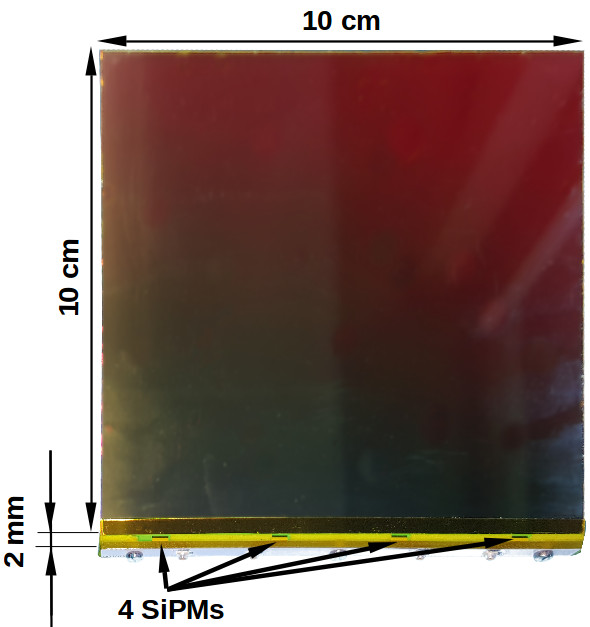
\includegraphics[width=.5\textwidth]{arclight/prototype}
	\caption[\SI{10 x 10}{\centi\metre} \glsentryshort{arclight} prototype]{%
		\SI{10 x 10}{\centi\metre} \acrshort{arclight} prototype.
		Four \acrshortpl{sipm} can be seen at the lower side, soldered to a narrow \acrshort{pcb} providing coaxial connectors for signal readout.
		The rest of the sensor area is dielectric.
	}
	\label{fig:arclight_prototype}
\end{figure}

Most of the following has been published in~\cite{arclight}.
The \AL{} aims to minimise the occupied volume while maximising the area coverage of \glspl{sipm}.
This is achieved by coupling them to a passive light collector.
As mentioned above, principles based on full reflection on a polymer-\lar{} interface are not suitable.
Instead, \AL{} is based on the light trapping principle of the \gls{arapuca} sensor~\cite{arapuca}.
It works by trapping the photons inside a cavity made of walls covered by a highly reflective materials.
One of the walls is formed of a dichroic film, a material transparent to certain wavelengths while highly reflective to others.
On the outside this film is coated with \gls{tpb}, which shifts the \lar{} scintillation light to the blue range, where the dichroic film is transparent.
The inside of the film is covered by a second \gls{wls}, shifting the light to green, which is reflected by the dichroic film and therefore trapped inside the cavity.
One or more \glspl{sipm} are mounted inside the cavity to collect the trapped photons.
\AL{} improves the \gls{arapuca} design by replacing the empty cavity with a solid transparent polymer sheet doped with a \gls{wls} dye.
This makes it substantially more robust and compact, especially when scaled up to larger areas.

\begin{figure}[tbp]
	\centering
	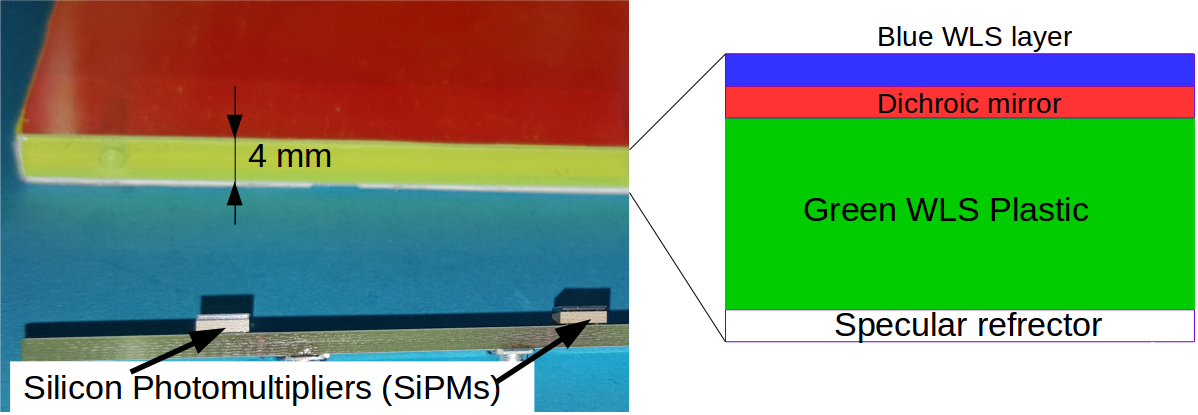
\includegraphics[width=\textwidth]{arclight/structure}
	\caption[\glsentryshort{arclight} light collector cross-section]{%
		\acrshort{arclight} light collector cross-section near a corner.
		The structure is mechanically supported by a \SI{4}{\milli\metre} thick \acrshort{wls} plastic.
		Its front is covered with a dichroic mirror film while the edges and the back face are covered with a dielectric specular reflector foil.
		The outer surface of the dichroic mirror is coated with \acrshort{tpb} to shift the \acrshort{lar} \acrshort{vuv} scintillation light to the blue range, where the dichroic film is transparent.
		At the bottom of the left picture two of the four \acrshortpl{sipm} mounted to the carrier \acrshort{pcb} are visible.
	}
	\label{fig:arclight_structure}
\end{figure}

A \SI{10 x 10}{\centi\metre} \AL{} prototype is shown in Figure~\ref{fig:arclight_prototype}.
The ratio of sensitive area to total area is \SI{98}{\percent} with the remaining \SI{2}{\percent} occupied by a \gls{pcb} carrying four \emph{Hamamatsu S13360-3050VE} \glspl{sipm}~\cite{arclight_sipm} with a sensitive area of \SI{3 x 3}{\milli\metre} each.
The inside of \AL{} is made of a \SI{4}{\milli\metre} thick \emph{Eljen Technology EJ-280} \gls{wls} plate~\cite{arclight_wls}.
Its sides are laminated with reflective films.
The back face and the edges are covered with a \emph{3M Vikuiti ESR} dielectric specular reflector foil~\cite{arclight_esr} having $\approx \SI{98}{\percent}$ reflectance in the visible light range.
A \emph{3M DF-PA Chill} dichroic mirror~\cite{arclight_dichroic} covers the front face.
It is transparent in the blue and has a high reflectance in the green spectral range.
Both films are held in place by thin layers of transparent adhesive.
To shift the \gls{vuv} scintillation light produced in \lar{} to the blue transparent range of the dichroic mirror its outer surface is coated with \gls{tpb}.
A cross-section of the structure of \AL{} is depicted in Figure~\ref{fig:arclight_structure}.

\begin{figure}[tbp]
	\centering
	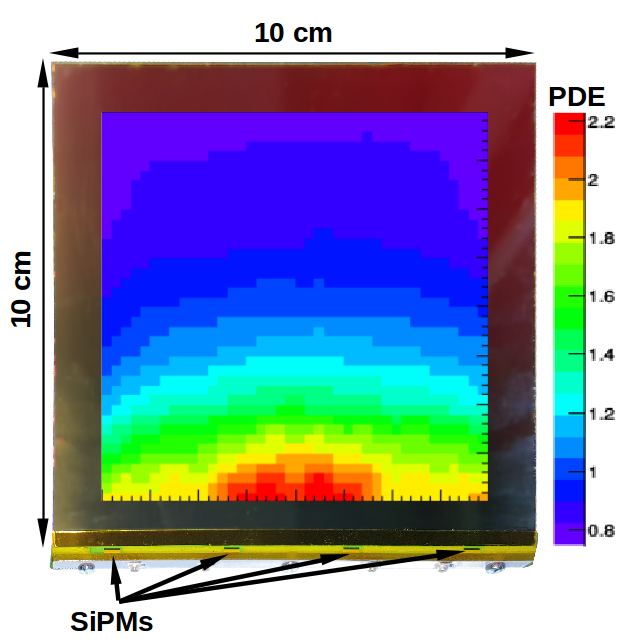
\includegraphics[width=\textwidth]{arclight/PDE}
	\caption[Measured \glsentryshort{arclight} \glsentryshort{pde}]{%
		Measured \acrshort{pde} for the \SI{10 x 10}{\centi\metre} \acrshort{arclight} prototype (in the background), at room temperature.
		The \acrshort{pde} is given in \si{\percent}.
	}
	\label{fig:arclight_pde}
\end{figure}

The \gls{pde} was measured at room temperature using an \ce{^{241}Am} source, previously calibrated with a \gls{pmt}.
A \gls{pde} of \SIrange{0.8}{2.2}{\percent} was measured.
Figure~\ref{fig:arclight_pde} shows \gls{pde} as a function of the position inside the light collector, overlaid on a picture of the prototype for reference.
The increase in \gls{pde} near the \glspl{sipm} is likely caused by photons hitting the \glspl{sipm} directly with no prior reflection off the dichoic mirror.
Due to the angular dependence of the dichroic mirror's reflectance about \SI{30}{\percent} of the light is lost during the first reflection on the mirror.
Once reflected, a photon is trapped inside the \AL{} because of the specular nature of the reflection on all surfaces.
Additionally, the average \gls{pde} was calculated from theory to be \SI{0.7 +- 0.4}{\percent}, in agreement with the measurements.
More details on the calculations and the calibration of the measurement can be found in~\cite{arclight}.

\begin{figure}[tbp]
	\centering
	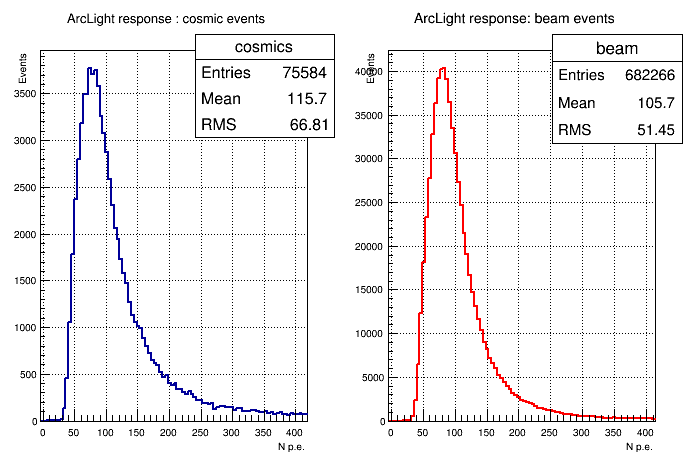
\includegraphics[width=\textwidth]{arclight/light_yield}
	\caption[\pixlar{} \glsentryshort{arclight} response]{%
		Distribution of observed number of photo-electrons (N p.e.)\ per event by the \acrshort{arclight} module in the \pixlar{} test beam demonstrator at \acrshort{fail}.
		The response is shown for cosmic (blue) and beam events (red).
	}
	\label{fig:arclight_pixlar_response}
\end{figure}

The measurements described above were performed at room temperature.
A \SI{43 x 15}{\centi\metre} \AL{} module was successfully operated at \lar{} temperatures in the \pixlar{} test beam demonstrator at \gls{fail}, described in Section~\ref{sec:ac_pixlar}.
Figure~\ref{fig:arclight_pixlar_response} shows the response for beam (red) and cosmic events (blue).
Cosmic events yield a mean of \num{115.7} photo-electrons while beam events produce slightly less light with a mean of \num{105.7} photo-electrons.
The time evolution of the mean photo-electron yield per event in beam (magenta) and cosmic ray (blue) mode is depicted in Figure~\ref{fig:arclight_pixlar_stability}.
Secondary beam energy and bending magnet current, selecting the momentum range of the tertiary beam, are also plotted for reference.
It can be seen that the photo-electron yield is approximately constant over several weeks.
The jumps in the response to beam events can be explained by the switching between different beam configurations.

\begin{figure}[tbp]
	\centering
	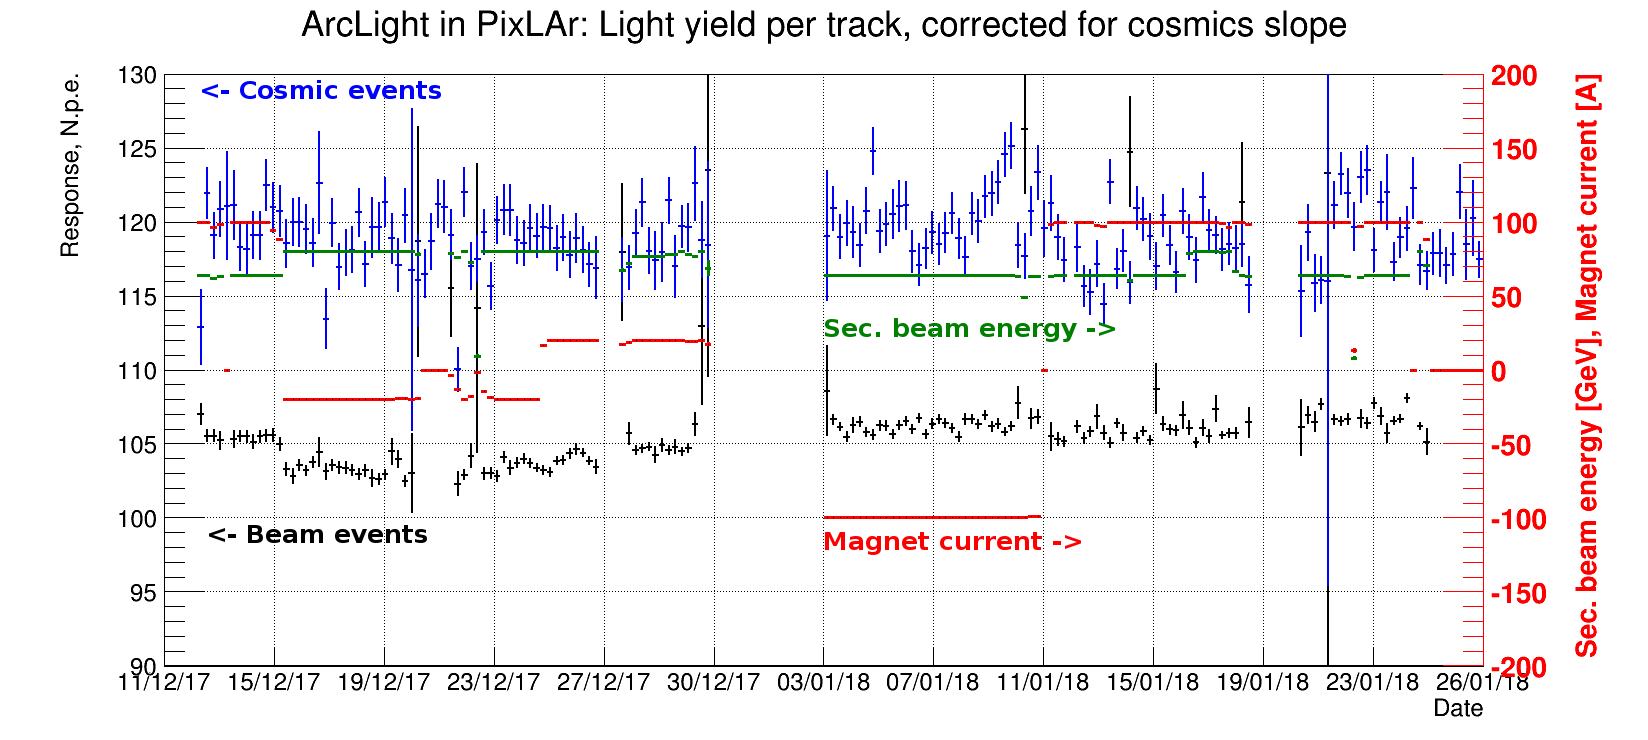
\includegraphics[viewport=0 0 1648 690, clip, width=\textwidth]{arclight/stability_cosm_beam_mod}
	\caption[\pixlar{} \glsentryshort{arclight} response stability]{%
		Mean observed number of photo-electrons (N p.e.)\ per event by the \acrshort{arclight} module in the \pixlar{} test beam demonstrator at \acrshort{fail}, over several weeks.
		The response is shown for cosmic (blue) and beam events (black).
		For reference the secondary beam energy (green) and the bending magnet current (red) are shown.
	}
	\label{fig:arclight_pixlar_stability}
\end{figure}


\section{Light Readout Summary}
\label{sec:studies_light-col-summary}

Classic \gls{pmt}-based light readout schemes for \lartpc{}s occupy large inactive volumes.
\glspl{sipm} are much smaller but so is their sensitive area.
I successfully used a cold \gls{sipm}-based light readout to trigger the charge readout of a pixelated \lartpc{} prototype.
\AL{} is a new light readout system based on the \gls{arapuca} light trap principle to increase the sensitive area of \glspl{sipm}.
Initial characterisations indicate a \gls{pde} of $\sim{\SI{1}{\percent}}$.
It can be installed inside the field cage of a \lartpc{} due to its low volume and the dielectric nature of the light collector.